% !TEX encoding = UTF-8
% !TEX TS-program = pdflatex
% !TEX root = ../nt.tex
% !TEX spellcheck = it-IT

%************************************************
\chapter{Appendici}
\label{cap:appendix}
%************************************************\\

\section{Esercizio (Core di Facebook)}

Analizziamo un esercizio riguardante il core di Facebook. Sul social network un autore ha la possibilità di scrivere dei Post ai quali possono essere aggiunti dei commenti o dei like, oppure possono essere condivisi da altri autori.  

Le prime entità che modelliamo sono la Persona e Post. 

\begin{center}
\begin{figure}[H]
\centering
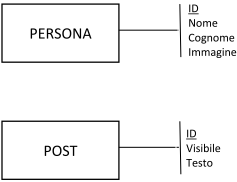
\includegraphics[scale=1]{figures/persona_post.png}
\caption{Entità Persona e Post}
\end{figure}
\end{center}

Cosa importante in Facebook sono i criteri di privacy per visualizzare i propri post. I criteri di privacy possono essere modellati come un tipo di entità oppure utilizzando il concetto di \textit{metadatabase}. Esso è un database che definisce le regole di funzionamento di un altro database. In pratica viene definita una regola che viene scritta all’interno nell’entità “Criteri di Privacy” e permette di far vedere il post solo agli amici o agli amici degli amici (è un pezzo di database che ha un’influenza sul database senza avere una propria entità, è detto \textit{meta-dato}).
  
Altre entità che andremo a modellare sono la Risorsa (rappresenta i riferimenti online che possono essere raggruppati in base al tipo), l’Album e il Gruppo.   

\begin{center}
\begin{figure}[H]
\centering
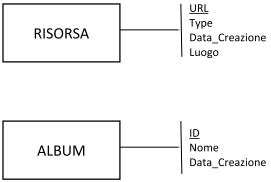
\includegraphics[scale=1]{figures/risorsa_album.png}
\caption{Entità Risorsa ed Album}
\end{figure}
\end{center}

\begin{center}
\begin{figure}[H]
\centering
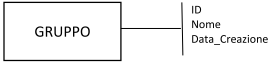
\includegraphics[scale=1]{figures/gruppo.png}
\caption{Entità Gruppo}
\end{figure}
\end{center}

Possono essere modellate due relazioni ricorsive su Persona e su Post:

\begin{center}
\begin{figure}[H]
\centering
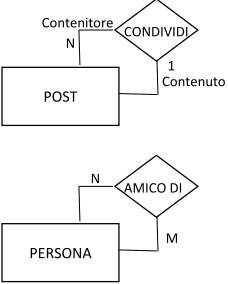
\includegraphics[scale=1]{figures/pap_pcp.png}
\caption{Relazioni: Post Condividi Post, Persona Amico Di Persona}
\end{figure}
\end{center}

Le relazioni che possono essere fatte tra Persona e Post sono:

\begin{center}
\begin{figure}[H]
\centering
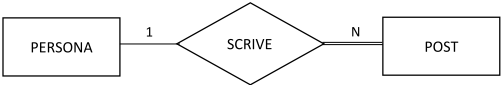
\includegraphics[scale=1]{figures/persona_scrive_post.png}
\caption{Persona Scrive Post}
\end{figure}
\end{center}

Notiamo che fra Post e Scrive è presente il vicolo di partecipazione totale.

\begin{center}
\begin{figure}[H]
\centering
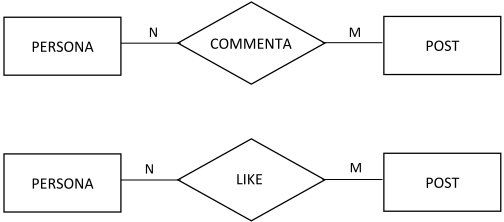
\includegraphics[scale=1]{figures/pcp_plp.png}
\caption{Persona Commenta Post, Persona Like Post}
\end{figure}
\end{center}

Invece tra Persona e Risorsa creiamo la relazione: 

\begin{center}
\begin{figure}[H]
\centering
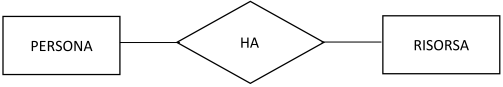
\includegraphics[scale=1]{figures/persona_ha_risorsa.png}
\caption{Persona Ha Risorsa}
\end{figure}
\end{center}

Tra Album e Risorsa è presente la relazione: 

\begin{center}
\begin{figure}[H]
\centering
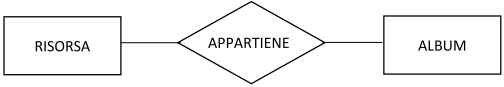
\includegraphics[scale=1]{figures/risorsa_appartiene_album.png}
\caption{Risorsa Appartiene ad Album}
\end{figure}
\end{center}

Inoltre è presente una relazione ricorsiva su Album, chiamata “Contiene” 

\begin{center}
\begin{figure}[H]
\centering
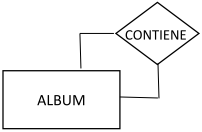
\includegraphics[scale=1]{figures/album_contiene_album.png}
\caption{Album Contiene Album}
\end{figure}
\end{center}

L’entità Gruppo viene collegata alla Persona con la relazione “Crea” e con la relazione “Si iscrive” (utilizzo il pattern \textit{Preventivo Consuntivo} per capire quando viene fatta la richiesta di iscrizione e quando viene accettato nel gruppo). 

\begin{center}
\begin{figure}[H]
\centering
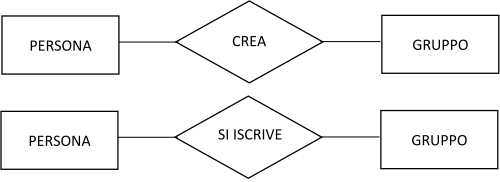
\includegraphics[scale=1]{figures/pcg_psig.png}
\caption{Persona Crea Gruppo, Persona Si Iscrive a Gruppo}
\end{figure}
\end{center}

Per ogni tipo di entità abbiamo almeno 2 tipi di vista, vista elenco (vengono distinte le persone online dalle persone generiche, o elenco solo degli amici) e vista di dettaglio. Lo schema finale del database sarà: 

\begin{center}
\begin{figure}[H]
\centering
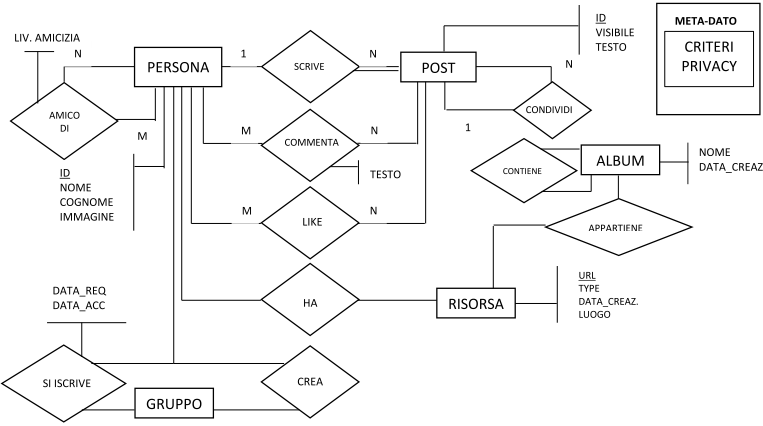
\includegraphics[scale=0.7]{figures/facebook.png}
\caption{Core di Facebook - ER Finale}
\end{figure}
\end{center}

Gli stakeholders in questo esempio saranno:

\begin{itemize}
\item Amministratore;
\item Utente;
\item Amministratore dei gruppi.   
\end{itemize}

\subsection{Esempi di interrogazioni}

\begin{itemize}
\item Dato un post fammi vedere quali commenti ha, chi ha scritto questi commenti, e quali altri commenti ha scritto uno stesso autore in altri post;
\item Dato un post fammi vedere quali commenti ha, chi ha scritto questi commenti, e quali altri post ha scritto uno stesso autore;
\item Dato un post condiviso, vedo il post originario e da chi è stato condiviso e la persona che è stato a condividerlo;
\item Persona amico di persona che ha scritto post in ordine di data (Questa query rappresenta la bacheca di facebook). 

\begin{lstlisting}[language=SQL]
SELECT POST.TESTO, COMMENTA.TESTO 
FROM   Persona AS p1, Amico_Di, Persona AS p2, POST, COMMENTA 
WHERE p1.ID = Amico_Di.ID_Richiedente AND    
   p2.ID = Amico_Di.ID_Richiesto   AND   
   POST.ID_Persona = P2.ID    AND   
   COMMENTA.ID_POST = POST.ID    AND   
   P1.Nome="Signore" AND p1.Cognome="X" 
\end{lstlisting}

\item Data una persona, chi è il suo “bersaglio” preferito? 

\begin{lstlisting}[language=SQL]
SELECT  p2.ID, p2.NOME, p2.COGNOME, COUNT 
FROM   PERSONA AS p1, COMMENTA.POST, PERSONA AS p2 
WHERE p1.ID = COMMENTA.ID_PERSONA AND
   COMMENTA.ID_POST = POST.ID  AND   
   p2.ID = POST.ID_PERSONA    AND   
   p1.NOME="X" AND p2 .COGNOME="Y"
GROUP BY p2.ID
\end{lstlisting}

\end{itemize}

\subsection{Meta-Database e Meta-Dati}

Riprendiamo il concetto di Meta-Database e Meta-Dati. Per ottenere su MySQL l’elenco dei database, delle tabelle o delle viste basta effettuare attraverso delle query in un database particolare. All’interno del database esiste infatti l’Information Schema, nel quale sono contenute tutte le informazioni relative alle tabelle e agli attributi.  Un meta-database non è altro che un database che descrive i dati di un altro oggetto (ad esempio di un altro database). Il data-catalog invece è l’insieme delle tabelle che descrivono i dati. È possibile realizzare anche un database per fare \textit{introspezione} dei dati, cioè un DB che è in grado di analizzare la propria struttura. Il problema dell’introspezione è che non sappiamo come servircene, la utilizziamo entro certi limiti.  


\section{Modellazione}

I modelli concettuali, logici e fisici vengono utilizzati per descrivere come realizzare delle applicazioni. Quando si realizza il diagramma entità relazioni in realtà si sta progettando anche il livello applicativo. Abbiamo utilizzato il modello Model-View-Controller che è molto vicino al concetto della 3-Layer-Architecture.  I passi da effettuare per realizzare il modello quindi sono:

\begin{itemize}

\item{Requirements}:

\begin{itemize}

\item Business Model Canvas (BMC) oppure E3Value $(E^3V)$ (Si definisce contest e problema);
\item Goal \& Stakeholder (Nell’esempio universitario gli Stakeholder sono lo Studente, il Professore e il Goal è la Laurea);
\item Requisiti (La soluzione del problema).
\end{itemize}

\item{Modellazione}:

\begin{itemize}

\item Hardware;
\item Rete;
\item Software:

\begin{itemize}

\item Presentation;
\item Business Rule;
\item Data (Enhanced Entity Relationship: in realtà è il primo passo da effettuare nella modellazione. Bisogna aggiungere delle annotazioni a questo diagramma riguardanti il dimensionamento della rete o dell’Hardware in base alle tabelle ottenute).
\end{itemize}

\end{itemize}

\item{Implementazione}: In un DB posso usare il CRUD o le TRANSAZIONI ACID, senza usare programmazione a oggetti. 

\end{itemize}

\subsection{Stima della dimensione del database}


\begin{center}
\begin{figure}[H]
\centering
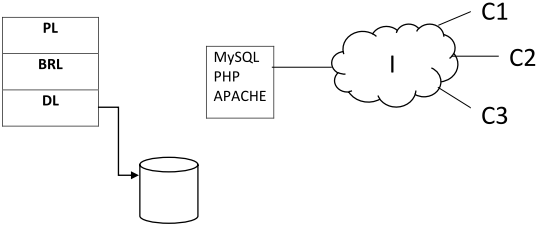
\includegraphics[scale=0.8]{figures/db_arch.png}
\caption{Architettura Logica DB}
\end{figure}
\end{center}

Il dimensionamento della rete e dell’Hardware (Ram, Disco, Macchine Virtuali) si ottiene in base alle tabelle e alle relazioni. 
  
Consideriamo ad esempio una semplice relazione:   

\begin{center}
\begin{figure}[H]
\centering
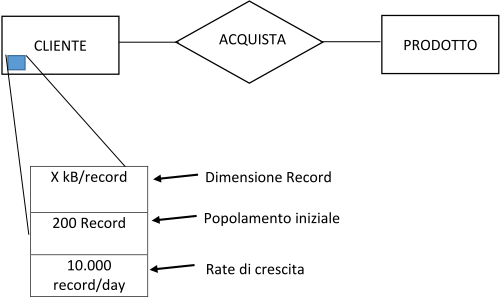
\includegraphics[scale=1]{figures/cap_dimensioning.png}
\caption{Cliente Acquista Prodotto - Dimensionamento}
\end{figure}
\end{center}

Tramite questi tre parametri indicati nella tabella il dimensionamento iniziale e la crescita successiva.

\begin{center}
\begin{figure}[H]
\centering
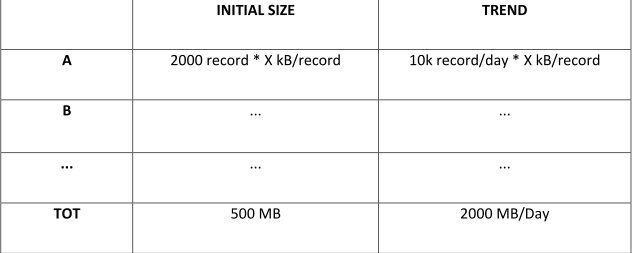
\includegraphics[scale=0.8]{figures/dimensioning_table.png}
\caption{Cliente Acquista Prodotto - Dimensionamento tabellare}
\end{figure}
\end{center}

Tramite questa tabella riusciamo a capire che dopo un anno il nostro Hardware avrebbe bisogno di 2 Terabyte. Questa tecnica quindi ci permette anche di stimare la banda media per ottenere un certo tempo di risposta durante il giorno della nostra macchina. 

\begin{center}
\begin{figure}[H]
\centering
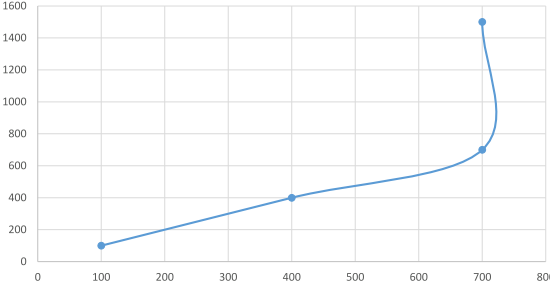
\includegraphics[scale=1]{figures/performance_plot.png}
\caption{Curva di Performance}
\end{figure}
\end{center}


\subsection{MODELLO VISIBILITY}

Per ogni Stakeholder presente è necessario disegnare il Visibility Model. Consideriamo nuovamente l’esempio precedente e realizziamo il visibility model per lo stakeholder 1 (S1): 

\begin{center}
\begin{figure}[H]
\centering
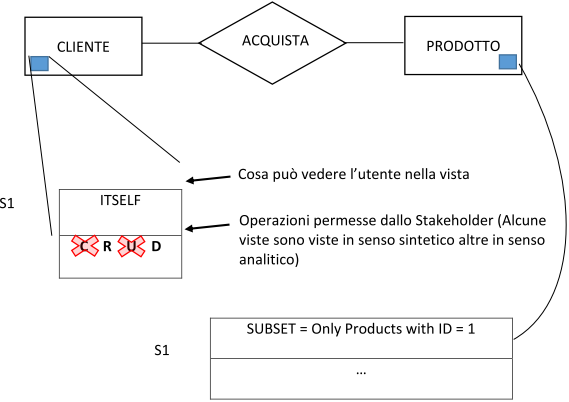
\includegraphics[scale=1]{figures/cap_visibility.png}
\caption{Modello Visibility di Cliente Acquista Prodotto}
\end{figure}
\end{center}

Anche in questo modello abbiamo due tipologie di navigazione:

\begin{itemize}

\item{IN THE LARGE NAVIGATION}: (Modello per mostrare le pagine e le connessioni fra di esse);
\item{IN THE SMALL NAVIGATION}: (Modello per analizzare ogni aspetto singolarmente, come i Menù, le voci, i bottoni). 

\end{itemize}



\begin{flushright}Angelo Cotardo\\Francesco Filieri\\13/03/2016\end{flushright}


\section{Esercizio (Compagnia Aerea)}

Si analizzi il seguente caso di studio:
Una nuova compagnia aerea vuole offrire un servizio di prenotazione e di acquisto di biglietti online, senza l’utilizzo alcuno di agenzie di viaggio né delle comuni biglietterie aeree ubicate presso gli aeroporti. Il sistema deve consentire le seguenti funzionalità:

\begin{itemize}

\item{IN FASE DI PRENOTAZIONE VIA INTERNET}:

\begin{itemize}

\item Consultazione degli orari e delle destinazioni dei voli disponibili;
\item Consultazione di eventuali offerte promozionali;
\item Scelta dell’orario e della destinazione;
\item Inserimento dei dati anagrafici dei passeggeri e delle eventuali preferenze (pasto, fumatori, ecc...);
\item Scelta del posto preassegnato (tenendo conto delle precedenti prenotazioni e delle preferenze);
\item Calcolo della tariffa da applicare (tenendo conto di eventuali offerte promozionali);
\item Addebito, previa conferma, del costo del biglietto sulla carta di credito fornita (sicurezza tramite protocollo SSL);
\item Stampa del biglietto elettronico che riporta il codice del biglietto i dati del/i passeggero/i, della partenza, della destinazione e il costo dettagliato (tariffa del biglietto, tasse, etc.).

\end{itemize}

\item{IN FASE DI CHECK-IN PRESSO L’AEREOPORTO DI PARTENZA}:

\begin{itemize}

\item Variazione del posto preassegnato (a seconda della disponibilità dei posti e delle precedenti prenotazioni e check-in);
\item Inserimento della segnalazione dei bagagli imbarcati;
\item Emissione della carta d’imbarco.

\end{itemize}

\item{IN FASE DI CONSUNTIVAZIONE VOLI}:

\begin{itemize}

\item Riscontro delle carte d’imbarco emesse;
\item Emissione di riepiloghi sui voli effettuati e sui passeggeri;
\item Analisi delle preferenze dei passeggeri ed invio di mailing mirate per informare di nuove promozioni e di servizi specifici per la clientela (ad esempio per viaggiatori che viaggiano spesso per vacanze in luoghi esotici, mailing per informarli di nuove destinazioni e di nuove offerte sulle loro rotte abituali).
\end{itemize}

\end{itemize}

Sulla base della seguente traccia, viene realizzato quello che è il modello E/R:

\newpage
\begin{center}
\begin{figure}[H]
\centering
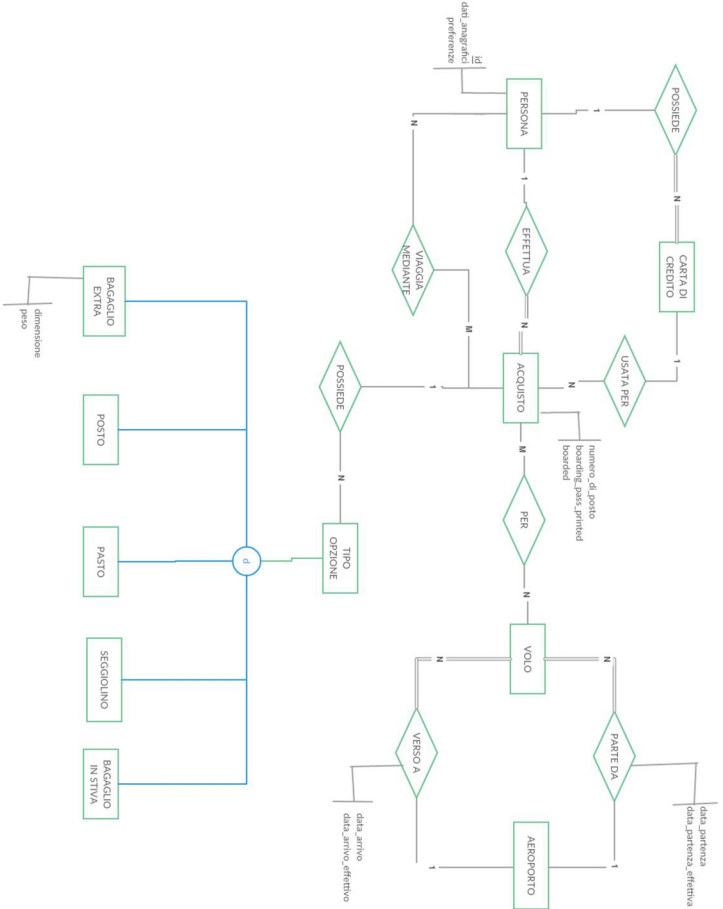
\includegraphics[scale=0.7]{figures/compagnia_aerea.png}
\caption{Compagnia aerea - ER Finale}
\end{figure}
\end{center}
\newpage

Nel diagramma riportato sopra si ha una possibile modellazione del caso di studio analizzato. La fase di modellazione è iniziata facendo riferimento all’azione principale che si deve compiere, cioè l’acquisto del biglietto aereo da parte del cliente.

Conviene non usare il termine biglietto, ma conviene scegliere un nome differente per evitare di creare problemi nel medio/lungo termine.

Perciò conviene usare un’entità che tenga traccia della transazione di acquisto, ed ecco perché si userà, come vedremo, l’entità acquisto.

Questo porta alla creazione di una relazione in cui le entità in gioco, come si può notare osservando la figura, sono:

\begin{itemize}

\item{\textit{Persona}};
\item{\textit{Acquisto}}.
\end{itemize}

Dato che una \textit{Persona} deve effettuare un \textit{Acquisto}, tenendo conto che gli acquisti possono essere eseguiti unicamente online, questa deve avere una o più \textit{Carte Di Credito} associate al suo profilo. È errato considerare la \textit{Carta Di Credito} come attributo di \textit{Persona} perché ad ogni individuo può essere associata più di una carta oppure potrebbe esserne sprovvisto, il che porterebbe ad avere un eccessivo numero di NULL nel database. Inoltre c’è la \textit{\textbf{PARTECIPAZIONE TOTALE}} dal lato della \textit{Carta Di Credito}, in questo modo ogni carta deve avere un titolare. Nel nostro modello E/R, non intendiamo l’entità \textit{Persona} solo come acquirente, ma viene intesa anche come passeggero, perché un utente può anche acquistare un biglietto per terzi.
In fase di \textit{Acquisto} è possibile selezionare delle opzioni, per tanto si è deciso di specializzare il \textit{Tipo Di Opzione} in modo da associare all’\textit{Acquisto} le varie proposte che la compagnia offre al cliente. Ad esempio:

\begin{itemize}

\item \textit{la selezione del posto};
\item \textit{l’aggiunta di un bagaglio extra con relative dimensioni e peso};
\item \textit{la selezione del tipo di pasto da consumare a bordo};
\item \textit{la presenza del bagaglio da portare in stiva};
\item \textit{la richiesta del seggiolino per bambini}.

\end{itemize}

L’entità \textit{Acquisto} ha come attributi necessari al soddisfacimento dei requisiti:

\begin{itemize}

\item \textit{numero di posto}, che è utile per tenere traccia del numero di biglietti già venduti e per far selezionare al cliente il posto desiderato o assegnarne uno casuale;
\item \textit{boarded\_pass\_printed, che è utile alla compagnia aerea per capire quanti passeggeri hanno stampato la carta d’imbarco e quindi il numero di persone che hanno intenzione di usufruire del volo};
\item \textit{boarded, che indica se la persona è effettivamente a bordo o meno}.

\end{itemize}

Come si intuisce facilmente, gli ultimi due attributi dell’entità \textit{Acquisto} saranno di tipo booleano. È stato scelto, inoltre, di modellare l’entità \textit{Volo}. Tale entità è in doppia relazione con l’entità \textit{Aeroporto}, in quanto, ciò ci permette di tenere traccia dell'\textit{Aeroporto} di partenza e quello di destinazione. Le due relazioni hanno come attributi:

\begin{itemize}
\item \textit{data prevista};
\item \textit{data effettiva}.
\end{itemize}

il che consente di monitorare eventuali ritardi e di avere un calendario completo dei voli. In una prima analisi si era deciso di creare un’entità Giorno, che era collegata in una relazione ternaria con le entità volo e aeroporto e le relazioni “parte da” - “verso”, allo scopo di creare un calendario dei voli. Questa procedura ha senso solo nel momento in cui l’entità giorno possiede diversi attributi che la caratterizzano o se il giorno deve contenere informazioni importanti (quindi si deve distinguere dagli altri giorni, come giorni da bollino nero, sconti per i festivi, ...), in modo da fornirle una certa dignità informativa, altrimenti se contiene semplicemente l’attributo data, allora la si considera come un attributo di una determinata entità o relazione. Infine c’è da gestire la questione degli scali, per poterlo fare si “gioca” con la cardinalità della relazione “\textit{per}” che collega gli attributi \textit{Acquisto} e \textit{Volo}.


\begin{flushright}Cristian Annicchiarico\\Mattia Marzano\\01/12/2016\end{flushright}

\begin{center}
\begin{figure}[H]
\centering
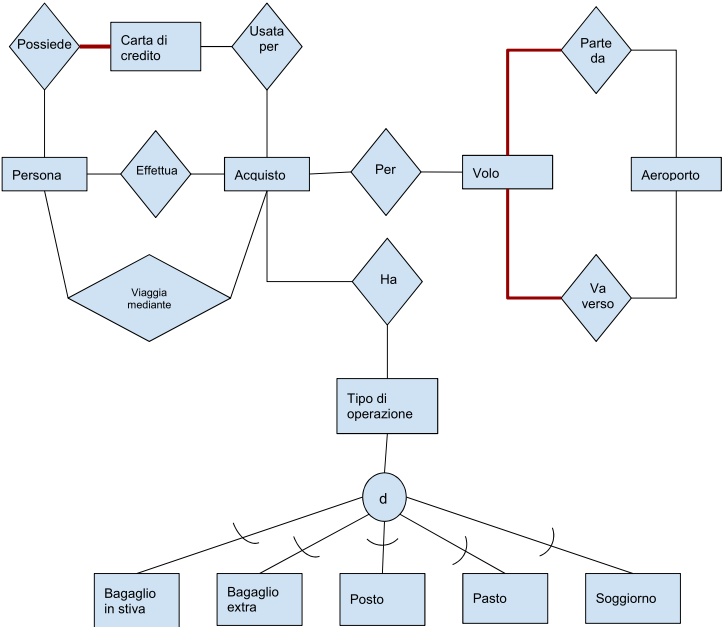
\includegraphics[scale=0.7]{figures/compagnia_aerea2.png}
\caption{Compagnia aerea - ER Finale - RECAP}
\end{figure}
\end{center}


\subsection{Continuazione ESERCITAZIONE}

Riprendiamo in esame lo scenario analizzato nella precedente lezione riguardante la gestione dei voli da parte di una compagnia.  Un’analisi più dettagliata ci ha permesso di cogliere delle problematiche che in prima approssimazione del modello relazionale non è stato possibile osservare. Il problema di questo schema si presenta principalmente con l’analisi della situazione in cui l’acquisto dei biglietti è multiplo. Qualora venisse effettuato un acquisto multiplo di biglietti, risulterebbe difficile l’implementazione dell’inserimento di un’opzione aggiuntiva da parte di un singolo cliente appartenente ad un gruppo, in modo indipendente.  Analizziamo più nel dettaglio cosa intendiamo per gruppo. Per gruppo in questo caso stiamo intendendo un agglomerato di persone. Vogliamo poter tenere traccia dei dati di ogni singolo passeggero, in quanto potrebbero essere potenziali clienti futuri per la compagnia di voli. Il problema fondamentale con il “gruppo” è: una persona che viaggia in gruppo può comprare un’opzione personale? Cerchiamo di modificare lo schema riportato sopra per risolvere il nostro problema.  

Ci possono essere almeno due modi generalmente validi per risolvere il problema:   

\begin{itemize}

\item{}

\begin{center}
\begin{figure}[H]
\centering
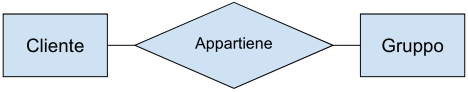
\includegraphics[scale=1]{figures/cliente_appartiene_gruppo.png}
\caption{Cliente Appartiene a Gruppo}
\end{figure}
\end{center}

Se consideriamo il primo schema per modellare un acquisto che si riferisce ad un gruppo di persone nel caso in cui un acquisto venisse effettuato da un cliente per una sola persona potremmo pensare che la tabella Gruppo presenti degli attributi a NULL. Riflettendo attentamente lo schema in figura 1 non vieta che il gruppo sia costituito da una sola persona pertanto non assistiamo alla presenza di NULL nella tabella Gruppo quanto ad una replicazione degli attributi di Cliente. In generale una schematizzazione siffatta è preferibile quando due oggetti sono eterogenei;

\item{}

\begin{center}
\begin{figure}[H]
\centering
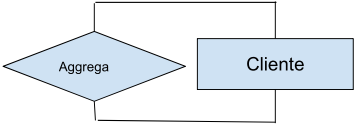
\includegraphics[scale=1]{figures/cliente_aggrega_cliente.png}
\caption{Cliente Aggrega Cliente}
\end{figure}
\end{center}

Con questo schema mettiamo in relazione l’entità Cliente con se stessa attraverso la relazione Aggrega. Notiamo che per i nostri propositi questa schematizzazione non va bene dal momento che Cliente e Gruppo non sono oggetti omogenei. In generale questo tipo di schematizzazione è preferibile quando gli oggetti sono omogenei; un esempio può essere una gerarchia di Persone come in un albero genealogico.

\end{itemize}


\subsubsection{Query SQL}

\begin{itemize}

\item Numero di CC della persona con nome Mario Rossi:

\begin{center}
\begin{figure}[H]
\centering
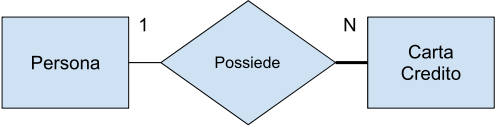
\includegraphics[scale=1]{figures/persona_possiede_cc.png}
\caption{Persona Possiede Carta di Credito}
\end{figure}
\end{center}

\begin{lstlisting}[language=SQL]
SELECT COUNT(*)
FROM PERSONA JOIN CARTACREDITO ON COD.PERSONA = ID.PERSONA
WHERE PERSONA.NOME = "Mario Rossi"   
\end{lstlisting}

\item Tutti i voli dell’aeroporto con nome “Aeroporto1”:

\begin{center}
\begin{figure}[H]
\centering
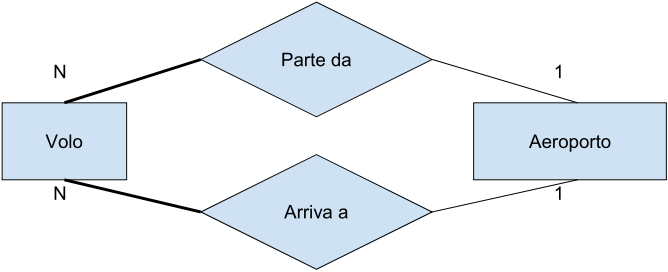
\includegraphics[scale=0.8]{figures/aereoporto_volo.png}
\caption{Volo Parte Da/Arriva A Aeroporto}
\end{figure}
\end{center}

\begin{lstlisting}[language=SQL]
SELECT *
FROM VOLO
JOIN AEROPORTO ON  VOLO.ID_AEROPORTO_PARTENZA = AEROPORTO.COD_AEROPORTO
WHERE AEROPORTO.NOME =  "Aeroporto1"
\end{lstlisting}

\item Estrazione della coppia di opzioni più acquistate (insieme):

\begin{lstlisting}[language=SQL]
SELECT MAX(CONTEGGIO), TO1.COD_OPZIONE, TO2.COD_OPZIONE
FROM (SELECT TO1.COD_OPZIONE, TO2.COD_OPZIONE, COUNT(*) AS CONTEGGIO 
FROM TIPO_OPZIONE AS TO1, TIPO_OPZIONE AS TO2 
WHERE TO1.COD_ACQUISTO = TO2.COD_ACQUISTO) 
\end{lstlisting}

OSSERVAZIONE: Sebbene questa query sia più articolata rispetto alle precedenti non si tratta di una subquery dal momento che la query annidata si trova nello statement FROM e non nel WHERE

\item Elenco di tutte le opzioni e del numero di volte che sono state vendute nell’anno 2016:

\begin{lstlisting}[language=SQL]
SELECT COUNT(*), TO.COUNT(*)
FROM TIPO_OPZIONE AS TO
JOIN INCLUDE AS I ON TO.COD_OPZIONE = I.ID_OPZIONE 
WHERE YEAR(INCLUDE.DATA) = 2016
GROUP BY TO.COD  
\end{lstlisting}

OSSERVAZIONE: Nello statement WHERE la condizione sulla data poteva essere scritta in termini di INCLUDE.DATA LIKE “\_ \_/\_ \_/2016”. Questa espressione non è sbagliata ma introduce operazioni di pattern matching che degradano le prestazioni della query. 

\end{itemize}


\subsection{DFM}

Partiamo dal Database OLTP transazionale, aggiungendo gerarchie spaziali, temporali e domain specific si costruisce il Database Multidimensionale e successivamente si individuano i fatti principali.  

\subsubsection{FATTI PRINCIPALI}

La determinazione dei fatti principali consiste nell’individuazione nel database riconciliato di quelle entità che sono interessate da un numero molto grande di transazioni. Nel nostro caso:  

\begin{itemize}

\item Acquisto;
\item In;
\item Richiede;
\item Scalo  
\end{itemize}

Prendiamo in considerazione il fatto “Scalo” i cui attributi sono Orario effettivo, Orario previsto e Tipo:   

\begin{center}
\begin{figure}[H]
\centering
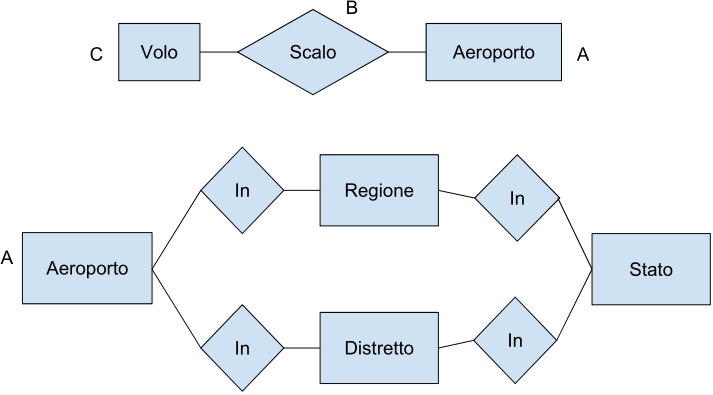
\includegraphics[scale=0.8]{figures/scalo_aeroporto.png}
\caption{Scalo FACT}
\end{figure}
\end{center}

\begin{itemize}

\item{A}: Da Aeroporto scaturisce una gerarchia spaziale per Scalo;
\item{B}: Dagli attributi Orario effettivo e Orario previsto scaturiscono gerarchie temporali:

\begin{center}
\begin{figure}[H]
\centering
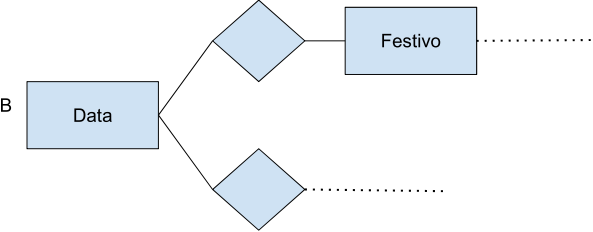
\includegraphics[scale=1]{figures/data.png}
\caption{Gerarchia ER - Data}
\end{figure}
\end{center}

\item{C}: Anche dall’entità Volo scaturisce una gerarchia relativa al fatto Scalo:

\begin{center}
\begin{figure}[H]
\centering
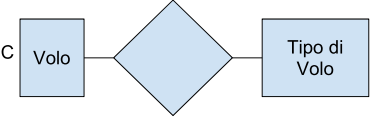
\includegraphics[scale=1]{figures/volo.png}
\caption{Gerarchia ER - Volo}
\end{figure}
\end{center}

\end{itemize}


\subsubsection{FACT MODEL}

Potrebbe essere interessante analizzare il fatto Decollo. Si noti che le misure rispetto cui il fatto è analizzato sono attributi calcolati, come ad esempio il numero dei passeggeri. 

\begin{center}
\begin{figure}[H]
\centering
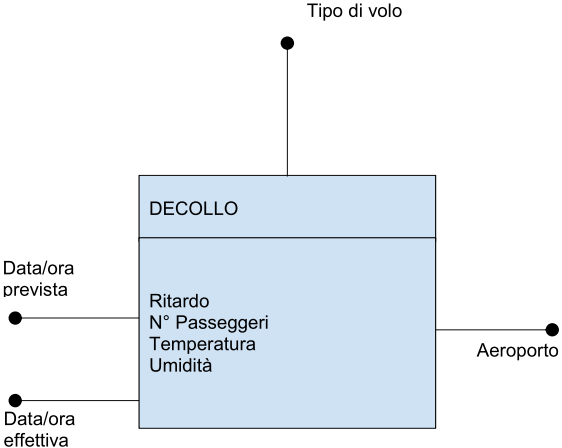
\includegraphics[scale=1]{figures/decollo.png}
\caption{Decollo FACT}
\end{figure}
\end{center}



\begin{flushright}Gabriele Accarino\\Emanuele Costa Cesari\\07/12/2016\end{flushright}


\section{DATABASE TECHNOLOGIES}


\subsection{CLOUD COMPUTING}

Il cloud computing è l’utilizzo di risorse digitali distribuite in maniera elastica usufruendo di Internet e serve per inquadrare big data e database NoSQL (Not only SQL). Quando parliamo di cloud presupponiamo di accedere a questo tramite protocolli HTTP o TCP-IP (dove per HTTP intendiamo il livello applicativo che poggia sul servizio di rete TCP-IP).  

Poiché col cloud computing la struttura non è fissa, la quantità di risorse utilizzate cambia dinamicamente: dal punto di vista del provider lo spazio viene redistribuito a seconda dei parametri economici e di servizio mentre da quello del client viene effettuata una richiesta a seconda della necessità. 

Il cloud computing ha così rilassato il concetto di dimensionamento ed allocazione delle risorse: quando andiamo a progettare un sistema non abbiamo più il bisogno di vedere preventivamente di quanto spazio, potere computazionale o banda necessita il nostro data center e comprarlo a priori. Infatti, i sistemi informatici, fino all’arrivo del cloud computing si sono basati sul concetto di massimo carico per il dimensionamento cercando poi di spalmare il costo delle risorse negli anni.  

Oggi, quindi, col cloud computing non ragioniamo più dimensionando sul picco, ma riallocando  la memoria in base alla richiesta media e contenendo gli eventuali picchi. Possiamo definire  dei parametri di servizio che dinamicamente possono fare aumentare la potenza di elaborazione  del server in modo che il data center sia in grado di gestire eventuali situazioni di carico. 

Dietro a questo nuovo scenario tecnologico c’è l’attuale modello di business (e.g. Gmail e servizi correlati). Abbiamo una serie di servizi gratuiti in cambio dei nostri dati che modellano la pubblicità: Google o qualsiasi altro provider vende le nostre info personali aggregate. 

Il cloud computing prevede tre tipologie: IaaS (Internet as a Service), PaaS (Platform as a Service), SaaS (Software as a Service). Con questi possiamo comprare storage e capacità computazionale:  non diventiamo possessori ma solo utilizzatori di questi oggetti, che sono regolati da un contratto di servizio. Questi contratti sono definiti SLA (service level agreement) e determinano la minima qualità del servizio erogato. Esistono inoltre paradigmi sul cloud computing: ad esempio il NIST americano dove vengono rappresentati i vari attori e le varie funzioni all’interno dell’architettura cloud. 

Un problema fondamentale è quello del posizionamento fisico dei dati per garantire la protezione della privacy degli stessi. La privacy, per legge, copre info su salute, minori, religione e sesso,  in tal modo possiamo determinare se un dato è riservato o è protetto da privacy e, quindi, anche il costo del dato stesso. Data protection o privacy sono elementi fondamentali quando si parla di cloud computing. 
Attualmente tutti i grossi provider di servizi stanno creando grossi data center cercando di portare sul cloud tutti i servizi critici commodity (servizi richiesti ma di pari qualità da parte di tutti  
i provider): per far ciò fanno uso di database distribuiti. Un database distribuito prevede che  i dati possano essere distribuiti geograficamente su più luoghi.  

Dobbiamo ad ogni modo avere un modello dati consistente per gestire come questi dati sono deployati tra i vari nodi. Ci sono tecniche per ottimizzare efficienza e gestione: un esempio può essere quello di considerare il database distribuito come centralizzato. Tuttavia, quando ci troviamo in un’ambiente distribuito di dati non possiamo verificare contemporaneamente tutte  le prerogative del mondo ACID (secondo la teoria di Brewer). 

Riportandoci al concetto di database di tipo transazionale, basato su modelli relazionali,  le transazioni devono essere ACID (Atomicity, Consistency, Isolation, e Durability). Il limite  delle relazioni è che funzionano benissimo quando parliamo di dati semplici, ma se facciamo uso  di file multimediali non vanno più bene le query: da qui è nato il mondo dei database Not only SQL: sono quei database che non hanno necessità di rispondere alle caratteristiche  delle transazioni ACID. 

Un’ultima, ma non meno importante, caratteristica del cloud computing è il multi-tenance:  data una infrastruttura permettiamo che ci siano diversi proprietari di dati. Questi però al momento della creazione del database possono decidere quali dati sono isolati e quali condivisi.


\subsection{NIST REFERENCE ARCHITECTURE}

Nel cloud computing abbiamo diversi attori: 

\begin{itemize}

\item{Cloud Consumer}: il principale stakeholder del servizio;
\item{Cloud Provider}: l’ente responsabile della disponibilità del servizio;
\item{Cloud auditor}: chi fa il monitoraggio dei servizi, performance, gestisce clausole degli SLA;
\item{Cloud broker}: chi effettua dei servizi di intermediazione tra domanda e offerta. 
Se gli SLA del servizio non sono garantiti, il broker avverte il provider del servizio.

\end{itemize}

\begin{center}
\begin{figure}[H]
\centering
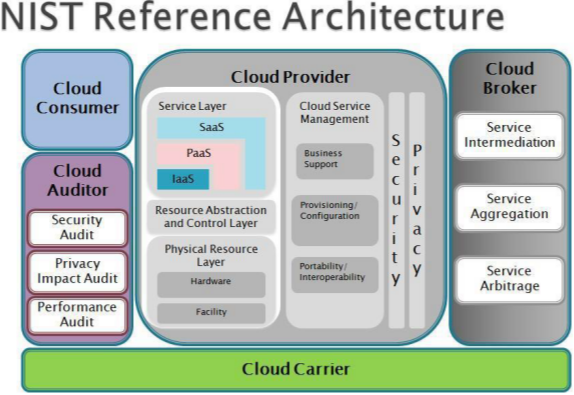
\includegraphics[scale=1]{figures/NIST.png}
\caption{Architettura NIST}
\end{figure}
\end{center}

\subsection{BIG DATA}


La crescita è stata esponenziale dalla nascita di internet: parliamo di “valanga di informazioni”  o peta bytes di dati che vengono gestiti. Quando ci riferiamo ai big data non badiamo solo al volume di dati ma anche ad altre caratteristiche particolari quali veridicità e velocità delle informazioni. 

Il famoso CRUD (Create, Read, Update, Delete) del database si applica a questa grossa mole  di dati che si più presentare in varie forme (infatti il tipo di visualizzazione è un tema abbastanza importante). È necessario quindi un sistema di “early warning” per fare l’analisi.

\subsection{CAP'S THEOREM}

Il teorema CAP, noto anche come teorema di Brewer, afferma che è impossibile per un sistema informatico distribuito fornire simultaneamente tutte e tre le seguenti garanzie: 

\begin{itemize}

\item{Coerenza}: (tutti i nodi vedono gli stessi dati nello stesso momento);
\item{Disponibilità}: (la garanzia che ogni richiesta riceva una risposta su ciò che è riuscito o fallito);
\item{Tolleranza di partizione}: (il sistema continua a funzionare nonostante arbitrarie perdite di messaggi).

\end{itemize}

Secondo il teorema, un sistema distribuito è in grado di soddisfare al massimo due di queste garanzie allo stesso tempo, ma non tutte e tre.  


\subsection{DATABASE NoSQL}

I database NoSQL (not only SQL) forniscono metodi di immagazzinamento e ricerca dati che sono modellati diversamente rispetto ai database relazionali, alcuni esempi sono: 

\begin{itemize}

\item{Key-value (k-v)}: formato da coppie chiave valore;
\item{Columnar}: formato perlopiù da colonne anziché righe;
\item{Document}: per gestire grosse moli di dati testuali (e.g., MongoDB o CouchDB);
\item{Graph}: formato da dati strutturati a grafo (e.g. Neo4J).
\end{itemize}


\subsection{MAP REDUCE}

MapReduce è un modello di programmazione per processare grandi set di dati. Si rifà alla struttura delle funzioni map e reduce utilizzate in programmazione funzionale. MapReduce è un framework per l'elaborazione di problemi parallelizzabili attraverso grandi dataset di dati che utilizzano un vasto numero di computer (nodi). L'elaborazione computazionale dei dati può essere o in un file system (non strutturato) o in un database (strutturato). Apache Hadoop è stato il primo sistema  di map reduce in parallelo. Spark ha successivamente sostituito Hadoop.  

\begin{itemize}

\item{Step "Map"}: Il nodo master prende l'input, lo divide in piccoli sotto-problemi, e distribuisce questi ai nodi computazionali. Questi ultimi possono ripetere a loro volta tale procedura, portando così  ad una struttura ad albero multilivello. A questo punto il nodo operativo elabora il problema più piccolo e poi passa la risposta al suo nodo master;
\item{Step "Reduce"}: Il nodo master raccoglie le risposte a tutti i sotto-problemi e li combina in qualche modo per formare la risposta al problema che sta cercando di risolvere. 

\end{itemize}



\begin{flushright}Federico De Luca\\Giuseppe D'Amuri\\15/12/2016\end{flushright}